\documentclass[paper=a4, fontsize=11pt]{scrartcl} % A4 paper and 11pt font size
\usepackage[T1]{fontenc} % Use 8-bit encoding that has 256 glyphs
%\usepackage{fourier} % Use the Adobe Utopia font for the document - comment this line to return to the LaTeX default
\usepackage[english]{babel} % English language/hyphenation
\usepackage{amsmath,amsfonts,amsthm} % Math packages
\usepackage{advdate} %other dates than today
\usepackage{sectsty} % Allows customizing section commands
%\allsectionsfont{\centering \normalfont\scshape} % Make all sections centered, the default font and small caps
\usepackage{geometry}
\usepackage{listings} %allows to print code
\usepackage[per-mode=symbol]{siunitx} %units (hertz)
\usepackage{graphicx} %allows images
\usepackage{epstopdf} %enables eps in pdfs
\usepackage{float} %fixes images
\usepackage{caption} %allows changing captions
\usepackage{polynom} %polynomial long division
%hobbled together long division?
\usepackage[display]{texpower}
%\usepackage{titlesec}


\newcommand{\ldsym}{$\left.\mathstrut\right)$}% unbalanced )
\newlength{\ldwidth}

\newcommand{\longdivide}[2]% #1 = denominator, #2 = numerator
{\settowidth{\ldwidth}{\ldsym}
$#1\,\raisebox{1.5pt}{\ldsym}\hspace*{-.65\ldwidth}\overline{
\mathstrut\hspace*{.35\ldwidth}\ #2}$}

\usepackage{fancyhdr} % Custom headers and footers
\pagestyle{fancyplain} % Makes all pages in the document conform to the custom headers and footers
\fancyhead{} % No page header - if you want one, create it in the same way as the footers below
\fancyfoot[L]{} % Empty left footer
\fancyfoot[C]{} % Empty center footer
\fancyfoot[R]{\thepage} % Page numbering for right footer
\renewcommand{\headrulewidth}{0pt} % Remove header underlines
\renewcommand{\footrulewidth}{0pt} % Remove footer underlines
\setlength{\headheight}{0pt} % Customize the height of the header

\setlength\parindent{0pt} % Removes all indentation from paragraphs

\setlength{\parskip}{.5cm} % space between paragraphs

%margins
\geometry{a4paper, top=1in, left=1in, right=1in, bottom=1.4in, includehead, includefoot}

%Don't number sections
%\renewcommand{\thesection}

%Don't bold section headings
%\sectionfont{}
%\subsectionfont{\textnormal}

\lstset{basicstyle=\ttfamily\small,xleftmargin=-1cm,xrightmargin=-2cm,breaklines=true} %settings and font for code

\usepackage[utf8]{inputenc}
\DeclareFixedFont{\ttb}{T1}{txtt}{bx}{n}{9} % for bold
\DeclareFixedFont{\ttm}{T1}{txtt}{m}{n}{9}  % for normal
% Defining colors
\usepackage{color}
\definecolor{deepblue}{rgb}{0,0,0.5}
\definecolor{deepred}{rgb}{0.6,0,0}
\definecolor{deepgreen}{rgb}{0,0.5,0}


\usepackage{listings}

% Python style for highlighting
\newcommand\pythonstyle{\lstset{
language=Python,
backgroundcolor=\color{white},
basicstyle=\ttm,
otherkeywords={self},            
keywordstyle=\ttb\color{deepblue},
emph={MyClass,__init__},          
emphstyle=\ttb\color{deepred},    
stringstyle=\color{deepgreen},
commentstyle=\color{red},
frame=tb,                         
showstringspaces=false            
}}

% Python environment
\lstnewenvironment{python}[1][]
{
\pythonstyle
\lstset{#1}
}
{}
\renewcommand{\thesubsection}{\alph{subsection}} %Lettered subsections
%\renewcommand{\thesubsubsection}{\roman{subsubsection}} %lower case roman numeral subsubsections

\renewcommand{\labelenumi}{\arabic{enumi}.}


\newcommand{\horrule}[1]{\rule{\linewidth}{#1}} % Create horizontal rule command with 1 argument of height

\DeclareMathOperator*{\argmin}{arg\,min} %argmin

\title{
\normalfont \normalsize
\huge The DoodleVerse \\ % The assignment title
}
\date{}

\begin{document}
\maketitle

\begin{figure*}[!h]
\center{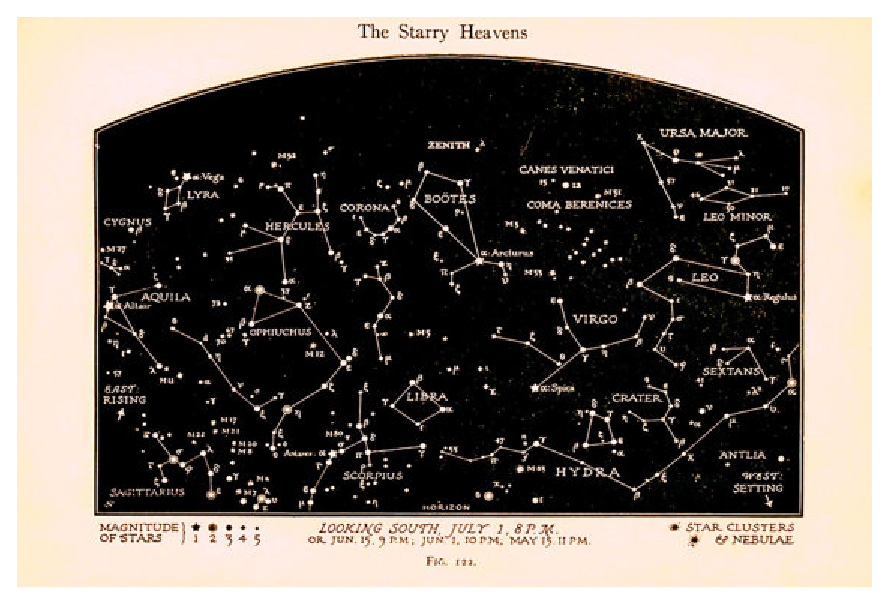
\includegraphics[scale=1]{space.eps}}
\captionsetup{labelformat=empty}
\caption{}
\end{figure*}

\section{Introduction}

Each civilization has their own set of constellations: groups of stars ascribed to a particular piece of cultural
memory. The ancient Greeks gave us most of our modern constellations. For example: Orion is a mythical
hunter. Could we take an arbitrary image and then find a set of stars that fit it? In this lab, we’ll
explore how to take a set of stars and construct spectacular celestial displays of your own
design. Welcome to the DoodleVerse!

\section{Overview}

The problem can be broken up into two main tasks: (1) taking the input image and extracting the ideal feature points, and (2) finding the ideal set of stars whose formation matches this set of feature points.

For the first task, we must perform a series of image processing steps to separate an image into a set of feature points. We must (a) define the image contours as sets of $k$ (x,y) coordinates that accurately depict the original image, and (b) reduce each contour into sets of $n<k$ (x,y) cooridinates that does not substantially degrade the original image representation. We do this by comparing the original contour to a linear spline connecting individual feature points and adding or removing points as necessary. 

For the second task, we start by framing it as an optimization problem. If $\mathbb{S}$ is our set of stars and $F$ is the matrix defined by our feature points, then we are looking for the subset $S\subset\mathbb{S}$ that minimizes the following: $||TF - S||_F$.  Here $T$ is a map from the Cartesian "feature space" to the space that our stars lie in that preserves the shape of our feature points (i.e. doesn't distort angles and relative distances).

The number of stars in our $\mathbb{S}$ set (which has been restricted to stars visible with the naked eye) is around 3000, so for $n$ feature points, there are around 3000 choose $n$ possibilities for $S$. The search space is too large for a brute force method.  We will proceed by breaking this problem into smaller problems to the point where a random search will yield sufficiently quick and accurate results. For this lab, we have provided you with a subset of $79$ stars.
\section{Warmup}

\subsection{Getting Feature Points}

In order to find a set of $n$ feature points of a drawing, we first need to turn the drawing into a set of contours from which we will get our feature points. In order to accomplish this, we need some form of edge detector. 

To detect edges in an image, you can think of them as large-amplitude changes in either the x-direction, the y-direction, or both. A standard way to do this is with the Sobel operator, which convolves an image with two $n$ by $n$ kernels, each of which is designed to detect changes in either the x or y axis. The general form of the result of applying this method to some matrix $A$ is $G = \sqrt{G_x^2 + G_y^2}$, where $G_x = \begin{bmatrix}
-1& 0 & 1\\
-2 & 0& 2\\
-1 & 0& 1
\end{bmatrix}\star A$ and $G_x =\begin{bmatrix}
-1 & -2 & -1\\
0 & 0 & 0\\
-2 & 0 & 2
\end{bmatrix} \star A$. You can implement each of these axis-specific operators using \texttt{scipy.ndimage.filters.sobel(A, mode='constant', ...)}, summing the squares of the results for \texttt{axis=0} and \texttt{axis=1}.

A more advanced border-following technique can be used for defining continuous contours\cite{Suzuki1985}. This technique is more useful than simple edge detection techniques because it determines an ordered contour instead of points of high "edge magnitude". The use of this technique is shown in Figure \ref{feat_detect}(b). 

\fbox{\begin{minipage}{40em}
\textbf{For a simple image, say a triangle with a black 1 pixel wide edge on a white background, suggest a reasonable edge detector to find the contour of the image. Why might a simple edge detector be "good enough" for this application?}
\end{minipage}}

Next, in order to narrow down our possible feature points, we can use a corner detector. Similar to how edge detectors look for large changes in particular directions, corner dectors look for large changes in more than one direction. One particular tool is the Harris Corner Detector.

Corners can be thought of as the intersection of two edges, so the gradient of the image will be large in both directions. In particular, if the function $I(x, y)$ represents the intensity of an image at position $(x, y)$, then we want to maximize $J(u, v) = \sum_{x,y} w(x, y) [I(x+u, y+v) - I(x, y)]^2$, where $w(x, y)$ is the window over which we’re looking at position $(x, y)$ and $(u, v)$ are the half-widths of the window in the $x$ and $y$ directions. After a Taylor expansion and some algebra, we can express $J$ as 

$$
J(u, v) \approx \begin{bmatrix}
u & v
\end{bmatrix} M \begin{bmatrix}
u\\
v
\end{bmatrix}
$$
where
$$
M = \sum_{x,y} w(x, y) \begin{bmatrix}
I_x^2 & I_x~I_y \\ I_x~I_y & I_y^2
\end{bmatrix}
$$

Now, for each window, a score $R$ is calculated and compared to a threshold value, to determine if a corner is present:
$$
R = [det(M) - k(Tr(M)]^2
$$
Furthermore, $det(M)$ and $Tr(M)$ can be expressed in terms of the eigenvalues $\lambda_1$ and $\lambda_2$: $det(M) = \lambda_1 \times \lambda_2$ and $Tr(M) = \lambda_1 + \lambda_2$. In summary, your results for Harris corner detection may still vary, depending on your choice of $u$, $v$, and $R$.

The local maxima from this approach yields the corners found in the image. By thresholding the $m > n$ largest-valued corners, the original set of $k >> n$ points can be largely reduced to a more manageable set of feature points as shown in Figure \ref{feat_detect}(c). This set can be fine tuned by additional methods to find better feature points. This is necessary because these $m$ feature points are not necessarily the most representative features of the contour. Many shapes may not give features that may seem obvious to us, so it is often useful to include a set of points that will exist for any contour so that the shape will at least have a minimal representation.  

\fbox{\begin{minipage}{40em}
\textbf{Given an arbitrary two-dimensional shape, determine some candidate feature points that will always exist.}
\end{minipage}}

Finally, in order to turn our $m$ feature points into the $n$ feature points that best represent the contour, we perform an algorithm which adds and removes points according to user-defined thresholds. We determine this set of $n$ points by testing points $p_{x_i},_{y_i}$ for how much their removal would induce error between the new contour $c_i$ and the original $k$ point contour $c^*$ by calculating the normalized absolute error $E$ between $c_i$ and $c^*$: $E = \frac{1}{|| p_{x_{i-1},y_{i-1}}  -  p_{x_{i+1},y_{i+1}} ||_2} \int\limits_{p_{x_{i-1},y_{i-1}}}^{p_{x_{i+1},y_{i+1}}} |l(x,y)| \ dx \ dy$ where $l(x,y)$ is the curve of $c^*$ relative to the linear spline connecting $p_{x_{i-1},y_{i-1}}$ and $p_{x_{i+1},y_{i+1}}$. The goal thus becomes to choose only those points that, for some theshold $T$, do not induce error $E > T$. The algorithm is defined below. Note that the order does not greatly affect the final result of the feature set and that the most important aspect is the selection of the threshold values $t_{delete}$ and $t_{add}$. 

\textbf{N-feature selection algorithm}
\\
(see Figure \ref{feat_detect}(d) for example of reducing an $m = 12$ point set to an $n = 8$ point set)
\begin{enumerate}
	\item 
	For all points $p_i$ in the set of $m$ features, find normalized error $E_i$ between $p_{i-1}$ and $p_{i+1}$. If $E_i < t_{delete}$, remove $p_i$ from the set of feature points. Else, move on to the next point. until all redundant points $j$ have been removed and your new set is composed of $y = m - j$ points.  
	\item
	For all points $p_i$ in the set of $y$ features, find normalized error $E_i$ between $p_{i}$ and $p_{i+1}$. If $E_i > t_{add}$, then add a new feature point along the contour at the bisecting point and test this new point to check if it meets the $t_{add}$ criterion. Else, move on to the next point. When finished, the new set of feature points is composed of $n = y + r$ points, where $r$ is the number of points added by this step. 
\end{enumerate}

\fbox{\begin{minipage}{40em}
\textbf{With the star dataset being used in this application taken into consideration, why is it so important to represent the shape in as few feature points as possible?}
\end{minipage}}

Finally, our approach that will be discussed later depends on picking three important initial feature points, so we must determine a good set of three points of the $n$ features that will give us a good chance at finding a match. This set of points will have well defined angles and large enough interpoint distances such that the three points do not line up with each other for form a line or near-line. Thus, the problem becomes a search for which three adjacent feature points along the contour best meet these requirements. In other words, which point solves the following: $p^* = max_{p_i} [ (||p_i - p_{i-1}||_2 + ||p_i - p_{i+1}||_2) sin(\theta_i) ]$ where $\theta_i$ is the angle spanning $p_{i-1}$ and $p_{i+1}$ going through $p_i$. An example of the key feature points is identified in Figure \ref{feat_detect}(d). 

\pagebreak

\begin{figure}
\center{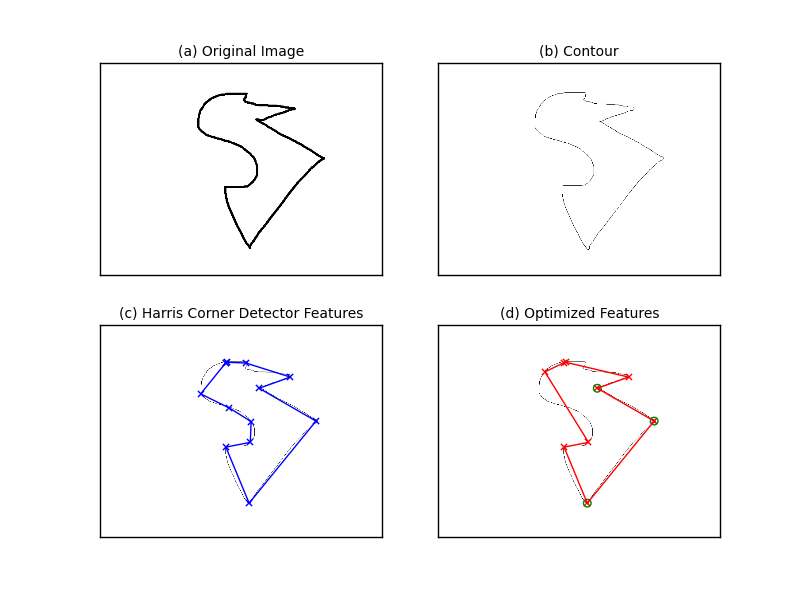
\includegraphics[scale=0.8]{feature_detection.png}}
\caption{(a) Original Image, (b) Contour of shape determined by \cite{Suzuki1985}, (c) Basic feature points determined by Harris Corner Detector, (d) Optimized feature points determined by thresholding algorithm with key feature points explicitly identified}
\label{feat_detect}
\end{figure}


\subsection{Cartesian and Spherical Coordinates: The Mollweide Projection}
Next we want to begin our search to see if we can find a set of stars that fits these feature points. The first issue we encounter is that our extracted feature points have Cartesian coordinates in the $(x,y)-$plane and our star data set is in spherical coordinates. Here is a readout of the first three stars of our raw data set:
\begin{python}
	   RA         Dec        Mag  
	float64     float64    float64
	---------- ------------ -------
	0.02662528 -77.06529438    4.78
	0.03039927  -3.02747891    5.13
	0.03266433  -6.01397169    4.37
\end{python}
The "RA" or "right ascension" measures the distance from a central meridian and ranges from $0$ hours to $24$ hours (which corresponds to $0\si{\degree}-360\si{\degree}$). To convert to degrees we need to multiply this column by $15$.
The "Dec" or "declination" measures the distances above or below the equator and ranges from $-90\si{\degree}$ to $90\si{\degree}$. The "Mag" or "magnitude" corresponds to the stars brightness. The scale is reversed: \textit{lower numbers correspond to brighter stars}.

The Mollweide (or homolographic) projection is a very useful projection for plotting objects in the night’s sky. Unlike most maps you’re used to seeing of the Earth’s surface, the Mollweide projection is ``equal-area”, meaning that the area enclosed within a given, closed curve is the same as the area enclosed within the Mollweide projection of that curve. Additionally, locally, the projection is flat, meaning that the un-projected data will look the same as the projected data if you zoom in far enough (realistically, this happens at scales of a few degrees). The Mollweide projection (and its cousin, the Hammer projection) have been used for about 30 years by the Cosmic Microwave Background physics community, who have used it to represent the temperature of the universe’s nearly-constant radiation field over the whole extent of the sky.  See Figure \ref{moll} for an example Mollweide projection.

\begin{figure}
\center{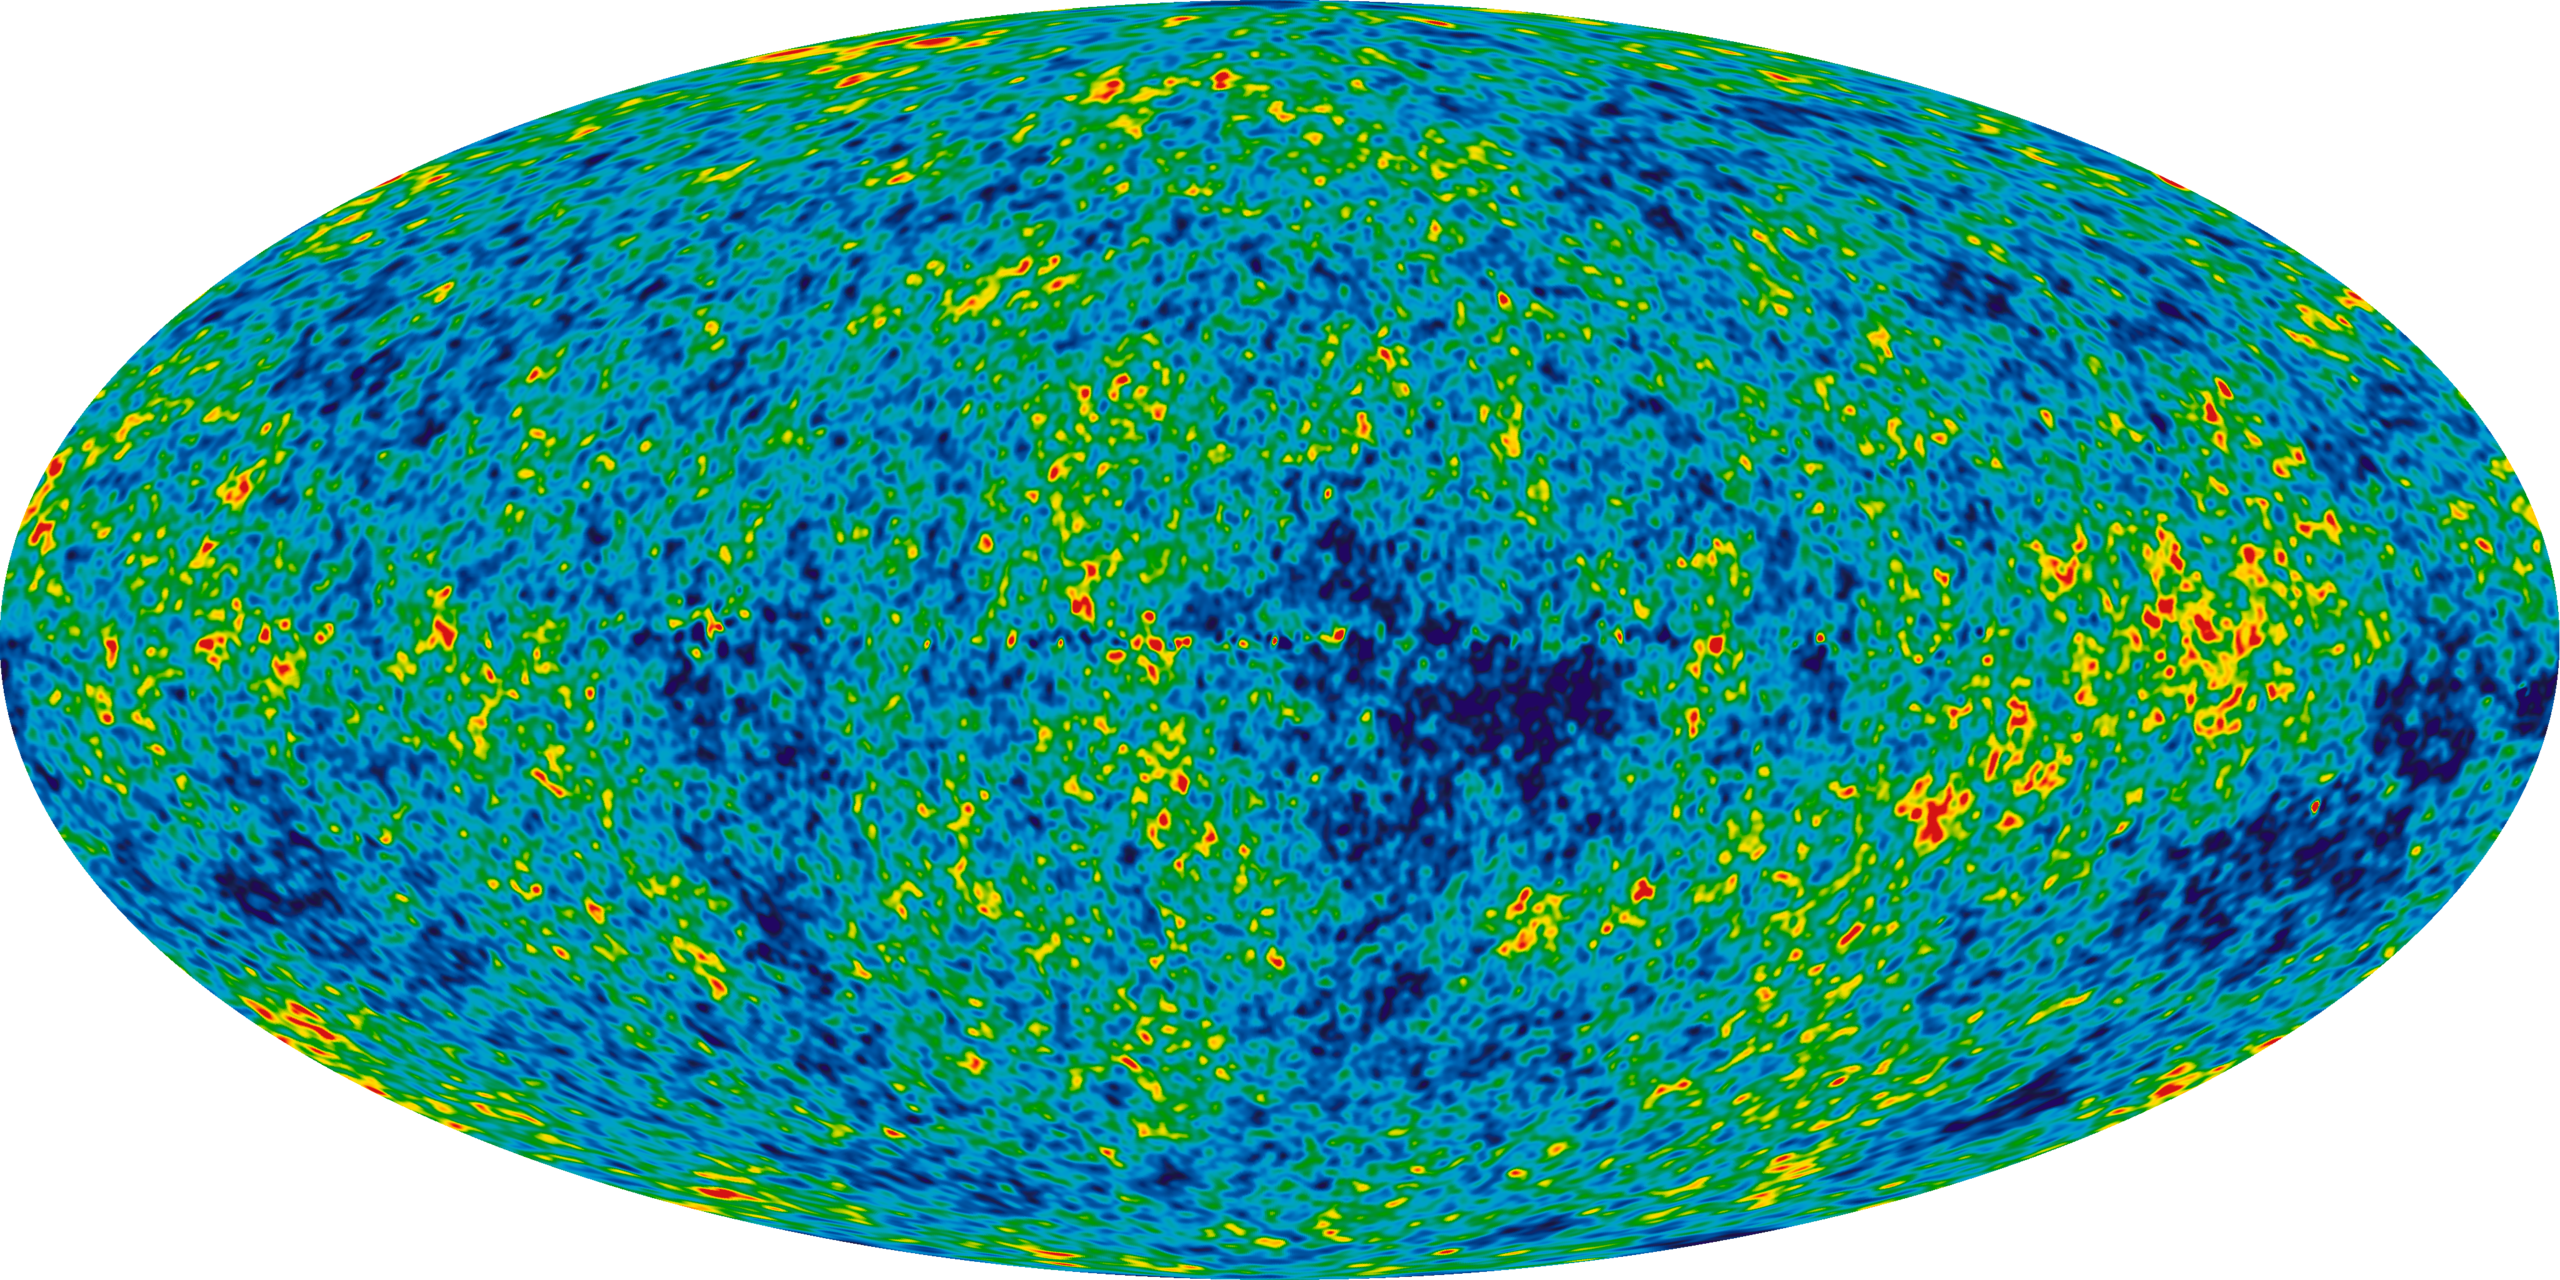
\includegraphics[scale=0.15]{mollweide.png}}
\caption{Mollweide projection of the temperature of the Cosmic Microwave Background Radiation (CMB), a nearly-uniform 2.7-Kelvin radiation source (Image: Wikipedia; Data: Wilkinson Microwave Anisotropy Probe)}
\label{moll}
\end{figure}


Functionally, the Mollweide projection has equally-spaced vertical parallels, but the meridians compress significantly near the poles, so that the whole unit sphere is represented as an ellipse with an axis ratio of two to one. We decided to use it here because of the tradition surrounding it, and also because it reduces to very little distortion at small spatial scales (on the order of a few degrees, the maximum scale over which we’ll form our constellations).

The Mollweide projection of a star with spherical coordinates $(\lambda,\phi)$ centered around ($\lambda_c,\phi_c$) can be obtained as follows \cite{Snyder1987}:
$$
x = R\frac{2\sqrt{2}}{\pi}(\lambda-\lambda_c)cos(\theta)$$$$
y = R\sqrt{2}sin(\theta)
$$
Where $\theta$ is the angle defined by: $2\theta + sin(2\theta)=\pi sin(\phi-\phi_c)$.  Since $\theta$ is implicitly defined, we cannot solve for it directly. But the following iteration will converge to its value after a few iterations (it converges slow for points far from our center point, but that is not a concern for us).
$$
\theta_0 = \phi-\phi_c
$$$$
\theta_{k+1} = \theta_k + \frac{2\theta_k+sin(2\theta_k)-\pi(sin\phi-\phi_c)}{2+2cos(2\theta_k)}
$$

Here is a Python script which will compute the Mollweide projection for given spherical coordinates:
\begin{python}

def project(ra, dec, c_ra, c_dec):
	'''
	Finds the Mollweide projection coordinates (x,y) for the point (ra,dec) around 
	point (c_ra,c_dec).
	'''
	
	# Find theta
	theta_0 = dec - c_dec
	epsilon = 10**-6
	error = 1+epsilon
	
	while error > epsilon:
	    m = (2*theta_0+np.sin(2*theta_0)-np.pi*np.sin(dec - c_dec))/(2+2*np.cos(2*theta_0))
	    theta_1 = theta_0 - m
	    error = np.abs(theta_1 - theta_0)
	    theta_0 = theta_1
	
	# Compute (x,y) coordinates
	x = 2*np.sqrt(2)*(ra-c_ra)*np.cos(theta_0)/np.pi
	y = np.sqrt(2)*np.sin(theta_0)
	
	return [x,y]
\end{python}

\fbox{\begin{minipage}{40em}
\textbf{Use this script to convert the 79 stars found in $stars.mat$ to (x,y) coordinates centered at ($\lambda_c,\phi_c)=(293, -2.8)$. (be sure to convert degrees to radians for the funcion defined above)}
\end{minipage}}

You should get something like this:
\begin{figure}[!h]
\center{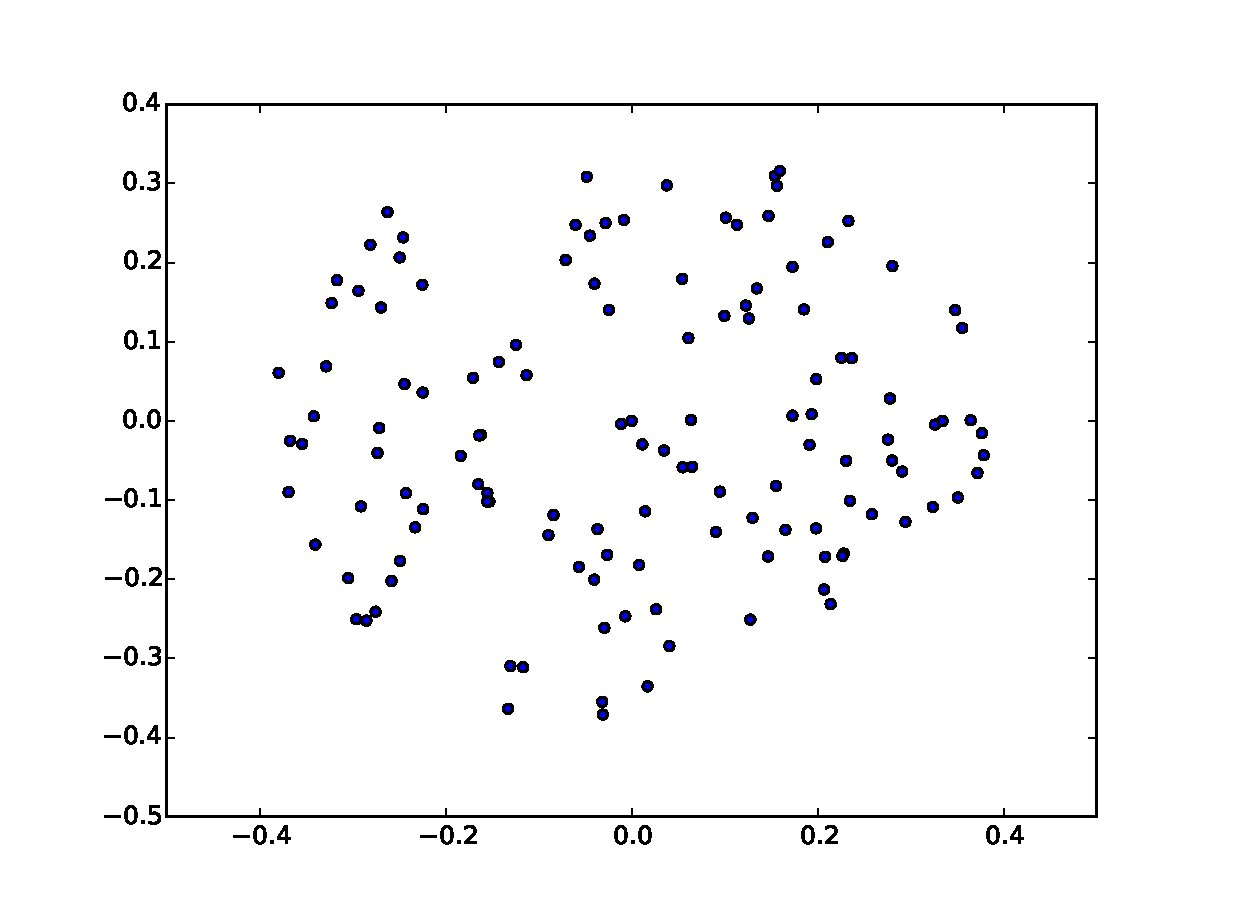
\includegraphics[scale=.7]{projection.eps}}
\captionsetup{labelformat=empty}
\caption{}
\end{figure}

\subsection{Preliminary Search: A Clustering Approach}
We wish to determine if there is possible good match for our feature points in the set obtained from the previous section.  Since we are only trying to match the shape and not the scale of our feature points, one approach is to find a set of stars that forms the same set of interior angles.

In essence, this is a clustering problem. First, let's simplify the problem by considering the case where our feature points consist of just 3 points: $(p_1,p_2,p_3)$. The shape of these 3 points is uniquely determined by their interior angles (i.e. the angles of the triangle they form), call them $(a_1,a_2,a_3)$. Finding these angles is a simple geometric formula:

The angle formed by $p_1, p_2, p_3$ with a vertex at $p_1$ is given by:

$$\arccos\left(\frac{P_{12}^TP_{13}}{||P_{12}||||P_{13}||}\right)$$

Where $P_{ij}$ is the vector formed by $(p_i - p_j)$.
The following script computes and the angles as we need them:

\begin{python}
def GetAngles(verts):
    '''
    Gets angles specified by points in verts,
    returns as a sorted array in radians.
    '''
    
    d = np.zeros((3))
    ab = verts[0]-verts[1]
    ac = verts[0]-verts[2]
    cb = verts[1]-verts[2]
    d[0] = np.linalg.norm(ab)
    d[1] = np.linalg.norm(ac)
    d[2] = np.linalg.norm(cb)
    
    a = np.zeros((3))
    a[0] = np.arccos(np.dot(ab,ac)/(d[0]*d[1]))
    a[1] = np.arccos(np.dot(ab,cb)/(d[0]*d[2]))
    a[2] = np.arccos(np.dot(ac,cb)/(d[1]*d[2]))
    
    return np.sort(a)
\end{python}

If we think of every set of 3 points in our search space as a specified by their interior angles (sorting the angles in ascending order uniquely determines the set's "angle representation"), we are basically looking for the 3-point sets that lie in the same cluster as our feature points. This cluster would be our "possible match" cluster.

\fbox{\begin{minipage}{40em}
\textbf{Form this as a clustering problem $X = DW$. What do $X,D,W$ look like? Our search set contains 79 stars. If D is $n\times k$, what is $n$? What would be the effect of choosing smaller or larger values of $k$?}
\end{minipage}
}

Unfortunately, even with our substantially restricted search space ($50-100$ stars), the number of possible size 3 subsets is still quite large (on the order of $10^4$), and the clustering algorithms we know require you to iterate through every point. Fortunately, it turns out that solving this cluster problem in its entirety is not necessary. We are not only looking for the \textit{best fit} sets of stars, we are looking for the best fit \textit{and brightest} sets of stars. By sorting the stars by magnitude, we can prioritize clustering the brightest stars so we find the brightest, best fits.

So if we are looking for $m$ possible matches in our subset, we can start with a much smaller subset of brightest stars and keep adding the next-brightest star until the cluster that contains our feature points has $m$ members.

This clustering approach is very valuable when searching over the whole set of stars. We can pre-compute the clustering for the combinations involving the brightest stars, and then just check which cluster our feature angles fall into to get a whole set of possible matches. For dealing with smaller search subspaces such as this one, it is actually pretty quick and efficient to just do a brute-force iteration through all possible star combinations in reverse order of brightness until we find a match that fits our features within a certain threshold. If we want $k$ possible matches, we just keep iterating until we find $k$ matches.

\fbox{\begin{minipage}{40em}\textbf{
This brute-force method only finds $k$ possible fits, where we choose $k$ ahead of time. Why might the clustering approach be more preferable?}
\end{minipage}}


Unfortunately, this approach doesn't scale well when our feature set is more than 3 points (most notably, the search space becomes way too large). However, matching 3 feature points to 3 stars does uniquely determine a transformation from the $(x,y)-$plane that the features lie in to the $(x,y)-$plane that the stars lie in. So rather than finding a match for the remaining points using this clustering approach, we can simply check to see if there are stars in the appropriate places to form the rest of our shape. To do this, we need to find the transformation from the $(x,y)-$coordinates of our features to the $(x,y)-$coordinates of our stars. To find this transformation, we must solve what is called the Procrustes problem.

\subsection{The Orthogonal Procrustes Problem\cite{Everson1997}}
Here we address the problem of finding the ideal transformation $T$ between our set of feature points $F$ and a predetermined subset of stars $S\subset \mathbb{S}$. Here we are assuming $F$ and $S$ are the same size $(2\times k)$ and represent their respective collections of points in Cartesian coordinates (each column is a point).  Finding this transformation will be necessary to evaluate the fitness of a possible match.

Other than minimizing the distance between points, the primary goal is preserving the shape of $F$. For now, let's also constrain the problem to where $S$ and $F$ are normalized, so we don't need to change the scale of $F$: our transformation will preserve distances and angles between points (and thus the shape). This simplifies the problem because it constrains $T$ to be orthogonal. Also, let's assume that both sets of points are centered around the origin (i.e. their mean is $\begin{bmatrix}
0\\
0
\end{bmatrix}$). Basically, we are looking for the best rotation of $F$ that minimizes the distance between its points and the points in $S$. Precisely, we are looking for the orthogonal $T$ that minimizes: 
$$||TF-S||^2_F = \langle TF-S, TF-S\rangle_F$$
Where $tr(AB^T) = \langle A,B\rangle_F = \langle B,A\rangle_F = tr(BA^T)$.

\fbox{\begin{minipage}{40em}\textbf{
Let $U\Sigma V^T$ be the SVD of the matrix $SF^T$. Show that the orthogonal $T$ that minimizes $||TF-S||^2_F$ is equal to $UV^T$.}\\
Hint: $T,U$, and $V$ are orthogonal, and multiplying a vector by an orthogonal matrix doesn't change its Frobenius norm.
Hint 2: If you're really stuck, check out \cite{Everson1997}
\end{minipage}}

Here is the Python code that solves the orthogonal Procrustes problem:

\begin{python}
def Procrustes(F, S):
	'''
	Given F, S (same size, unit norm, and centered around the origin), finds the
	ideal transformation that maps the points of F to best fit the points of S.
	That is, ||TF-S|| is minimized.
	'''
	
	[U,s,VT] = np.linalg.svd(np.dot(S,F.T))
	
	T = np.dot(U,VT)
	
	return T
\end{python}

\fbox{\begin{minipage}{40em}
\textbf{Use the Procrustes algorithm to find the transformation that best maps the $A$ to $B$ matrix found in the $procrustes.mat$ file.}
\end{minipage}
}

\subsection{Evaluating the Match}

Now we have sufficient machinery to evaluate our possible match.  We know we have a decent match for three of our feature points, and we know how to transform these feature points so they best align with the match. We just have to determine if there is decent match for the remaining feature points. To do this, we apply the same transformation to these feature points, and search for bright stars nearby the transformed points. In the simplest case, we could just pick the closest star to each transformed point and implement some cost function that penalizes dim stars.

Now we have our set of feature points $[f_1,\ldots,f_n]=F$, our possible match set of stars $[s_1,\ldots,s_n] = S$, with $[m_1,\ldots,m_n] = M$ being the set of magnitudes for the stars in $S$.

\fbox{\begin{minipage}{40em}\textbf{Suppose we had $k$ such possible matches $\{S_i,M_i\}$, and we want to determine the \textit{best} one. Set up a cost/penalizer function that we are trying to minimize.}
\end{minipage}}



\section{Lab}
You have been supplied: diamond.png (see Figure \ref{diamond}) and a subset of our star dataset $stars.mat$. Perform the following: 

\begin{figure}[!h]
\center{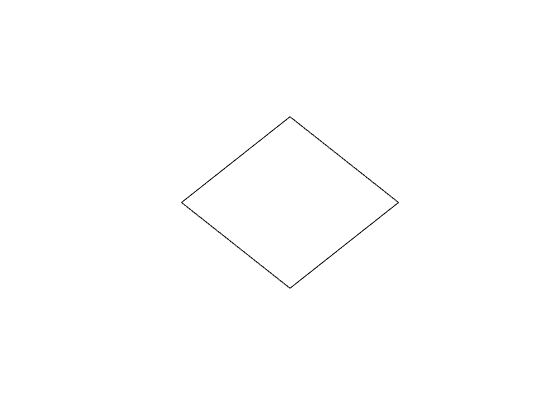
\includegraphics[scale=0.5]{diamond.png}}
\caption{diamond.png}
\label{diamond}
\end{figure}

\begin{enumerate}
  \item
  Import diamond.png to your program of choice (MATLAB or Python). Implement the edge detector of your choice to get a set of $k$ feature points that represent the shape. 
  \item 
  Implement a methodology to reduce this set of $k$ feature points to $n << k$  points. 
  \item
  Pick $3$ of your $n$ points and compute the angles between them. Now find a good potential match in (star-subset) for the triangle formed by these 3 points. Iterate through all possible combinations of stars in descending order of brightness until 3 "good" matches have been found.
  \item
  Generalize the orthogonal procrustes problem so that it will be useful for this case. That is, given the $(2\times k)$ matrix of feature points $F$ and a  $(2\times k)$ matrix of star points $S$ (which are not unit norm or centered around the origin), find ideal transformation $T$ such that $||T(F)-S||_F$ is minimized.  Note that it is easy to reduce to the previous case by computing the following:
  $$
  \hat{F} = \frac{F}{||F||_F} - mean(F)\quad\textrm{ and }\quad\hat{S} = \frac{S}{||S||_F} - mean(S)
  $$
  and solving the problem for $\hat{F}$ and $\hat{S}$. Modify the previous Procrustes problem code to solve the general Procrustes problem, and use it to map all of your $n$ feature points to the subspace containing the star projections.
  \item
  For the feature points that weren't part of your triangle, find the closest stars to their transformed positions. Repeat this process for your other good matches and evaluate the overall fit of your matches using your cost function from the previous section. Which match is best? If your cost function had a weighted penalizer for the star magnitude, how does changing this weight affect your evaluation?
\end{enumerate}

\bibliography{cited_papers}
\bibliographystyle{ieeetr}


\end{document}